\section{Deterministic finite state automata}

\begin{definition}
    A \emph{finite deterministic automaton M} consist of five elements:
    \begin{enumerate}
        \item $Q$, the state set (finite and not empty). 
        \item $\Sigma$, the input or terminal alphabet
        \item $\delta:(Q \times \Sigma) \rightarrow Q$, the transition function.
        \item $q_0 \in Q$, the initial state. 
        \item $F\subseteq Q$, the set of final states.
    \end{enumerate}
\end{definition}

The transition function encodes the automaton moves: 
\[\delta(q_i,a)=q_j\]
This notation indicates that when $M$ is in the current state $q_i$ and reads the input symbol $a$, it switches the current state to $q_j$. 
If $\delta(q_i,a)$ is undefined, then $M$ enters an error state and rejects the input string. 
The general transition function has the following domain $Q \times \Sigma^{*}$, and it is defined as:
\[\delta(q,ya)=\delta(\delta(q,y),a) \:\:\:\:\:\: \textnormal{where } a \in \Sigma \textnormal{ and }y \in \Sigma^{*}\]

\begin{definition}
    A string is \emph{recognized} if and only if, when the automaton moves through a path labeled by $x$, it starts from the initial state and ends at one of the final states: 
    \[\delta(q_0,x) \in F\]
\end{definition}
Note that the empty string is accepted if and only if the initial state is final as well. 
\begin{definition}
    The languages accepted by such automata are called \emph{finite-state recognizable}: 
    \[L(M)=\{x \in \Sigma^{*}|x \textnormal{ is recognized by } M\}\]
    
    Two automata are \emph{equivalent} if they accept the same language.
\end{definition}
The time complexity of finite state automata is optimal: the input string $x$ is accepted or rejected in real-time. 
Since it takes exactly as many steps to scan the string from left to right, the recognition time complexity could not be lower than this.

\subsection*{Error state and total automata}
If the move is not defined in state $q$ when reading character $a$, we say that the automaton falls into the error state $q_{err}$:
\[\forall q \in Q \forall a \in \Sigma \textnormal{ if } \delta(q,a) \textnormal{ is undefined then set } \delta(q,a)=q_{err}\]
It is always possible to complete the deterministic automaton by adding the error state, without changing the accepted language. 

\subsection*{Clean automata}
An automaton may contain useless parts not contributing to any accepting computation, which are best eliminated.
\begin{definition}
    A state $q$ is \emph{reachable} from state $p$ if a computation exists going from $p$ to $q$.

    A state is \emph{accessible} if it can be reached from the initial state. 

    A state is \emph{post-accessible} if a final state can be reached from it. 

    A state is called \emph{useful} if it is accessible and post-accessible. 

    An automaton is \emph{clean} if every state is useful.
\end{definition}
\begin{property}
    Every finite state automaton has an equivalent clean form.
\end{property}    
To reduce an automaton: first identify all the useless states, then strip them off the automaton along with all their incoming and outgoing arcs. 

\subsection*{Minimal automata}
\begin{property}
    For every finite state language there exists one, and only one, deterministic finite state recognizer that has the smallest possible number of states, which is called the minimal automaton.
\end{property}   
\begin{definition}
    The states $p$ and $q$ are \emph{undistinguishable} if, and only if, for every string $x \in \Sigma^{*}$, either both states $\delta(p,x)$ and $\delta(q,x)$ are final, or neither one is. 
\end{definition}
Two undistinguishable states can be merged and thus the number of states of the automaton can be reduced, without changing the recognized language.
Undistinguishability as a relation is symmetric, reflexive, and transitive. 
\begin{definition}
    The states $p$ and $q$ are \emph{distinguishable} if, and only if:
    \begin{enumerate}
        \item $p$ is final and $q$ is not or vice versa. 
        \item $\delta(p,a)$ is distinguishable from $\delta(q,a)$.
    \end{enumerate}
\end{definition}
\begin{example}
    Consider the following deterministic automaton: 
    \begin{figure}[H]
        \centering
        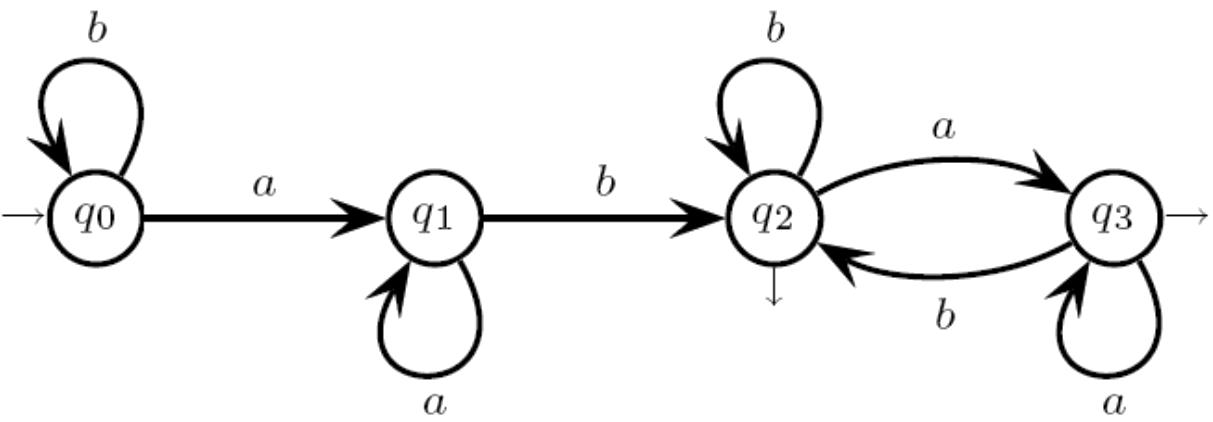
\includegraphics[width=0.5\linewidth]{images/fsamin.png}
    \end{figure}
    The corresponding undistinguishability table is as follows: 
    \begin{table}[H]
        \centering
        \begin{tabular}{cclcccc}
        \cline{2-3}
        \multicolumn{1}{c|}{\multirow{2}{*}{$q_1$}} & \multicolumn{2}{c|}{(1,1)}                     &                        &                       &              &             \\
        \multicolumn{1}{c|}{}                       & \multicolumn{2}{c|}{(0,2)}                     &                        &                       &              &             \\ \cline{2-5}
        \multicolumn{1}{c|}{\multirow{2}{*}{$q_2$}} & \multicolumn{2}{c|}{\multirow{2}{*}{$\times$}} & \multicolumn{2}{c|}{\multirow{2}{*}{$\times$}} &              &             \\
        \multicolumn{1}{c|}{}                       & \multicolumn{2}{c|}{}                          & \multicolumn{2}{c|}{}                          &              &             \\ \cline{2-7} 
        \multicolumn{1}{c|}{\multirow{2}{*}{$q_1$}} & \multicolumn{2}{c|}{\multirow{2}{*}{$\times$}} & \multicolumn{2}{c|}{\multirow{2}{*}{$\times$}} & \multicolumn{2}{c|}{(3,3)} \\
        \multicolumn{1}{c|}{}                       & \multicolumn{2}{c|}{}                          & \multicolumn{2}{c|}{}                          & \multicolumn{2}{c|}{(2,2)} \\ \cline{2-7} 
                                                    & \multicolumn{2}{c}{$q_1$}                      & \multicolumn{2}{c}{$q_2$}                      & \multicolumn{2}{c}{$q_3$} 
        \end{tabular}
    \end{table}
    From the table is possible to see that the only undistinguishable states are $q_2$ and $q_3$.
\end{example}

\subsection*{Minimization}
The minimal automaton $M^{'}$, equivalent to the given $M$, has for states the equivalence classes of the indistinguishability relation. 
To define the transition function of $M^{'}$, it suffices to state that there is an arc from class $C_1=[\dots,p_r,\dots]$ to class $C_2=[\dots,q_s,\dots]$ if and only if in $M$ there is an arc from state $p_r$ to $q_s$ wit the same label: 
\[p_r \overset{b}{\rightarrow}q_s \Leftrightarrow C_1=[\dots,p_r,\dots] \overset{b}{\rightarrow} C_2=[\dots,q_s,\dots]\]
That is, there is an arc between two states belonging to the two classes.
\begin{example}
    Consider the automaton from the previous example, it can be minimized by merging the two undistinguishable states that are found in the undistinguishability table. 
    The final automaton is the following: 
    \begin{figure}[H]
        \centering
        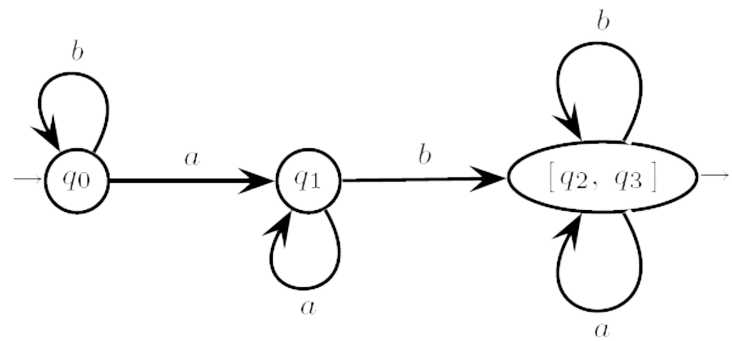
\includegraphics[width=0.5\linewidth]{images/fsamin1.png}
    \end{figure}
\end{example}